% Author:: Sebastien Badia (<seb@sebian.fr>)
% Date:: 2014-04-02 01:36:20 +0200
% vi: set ft=tex :

\section{Deploy, learn and tips}
\begin{frame}{Outline}
    \tableofcontents[currentsection,hideallsubsections]
\end{frame}

\begin{frame}{Development}
  \begin{textblock}{}(8,6)
    \includegraphics[height=1.8cm]{img/logo-git.png}
  \end{textblock}
  \begin{textblock}{}(11.5,-3)
    \includegraphics[height=2.5cm]{img/cat_review.jpg}
  \end{textblock}
  \begin{itemize}
    \item Integrated with launchpad (bug, milestone, cas)
    \item Code-review \url{https://review.openstack.org/}
      \begin{itemize}
        \item Git-review\footnote{\url{http://www.mediawiki.org/wiki/Gerrit/git-review}} (patch set lists / project setup / ease submit)
        \item In console, fgerrit\footnote{\url{https://github.com/pandemicsyn/fgerrit}}
      \end{itemize}
    \item Status \url{http://status.openstack.org/zuul/}
    \item Docs \url{http://wiki.openstack.org}
    \item IRC (oftc and freenode)
  \end{itemize}
\end{frame}

\begin{frame}{Git vs. Gerrit}
\vspace{-0.2cm}
\begin{center}
  \textbf{Git workflow}
\end{center}
\vspace{0.2cm}
\begin{center}
  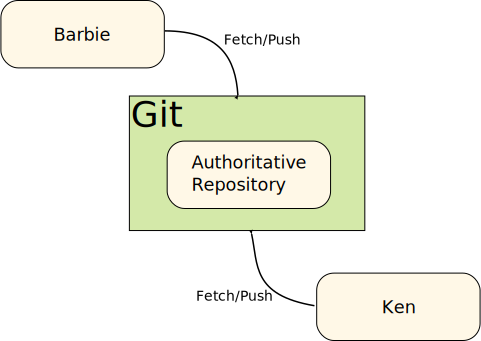
\includegraphics[height=6cm]{img/gerrit-workflow-classic.pdf}
\end{center}
\end{frame}

\begin{frame}{Git vs. Gerrit}
  \begin{center}
\textbf{Gerrit workflow}
\end{center}
\begin{center}
  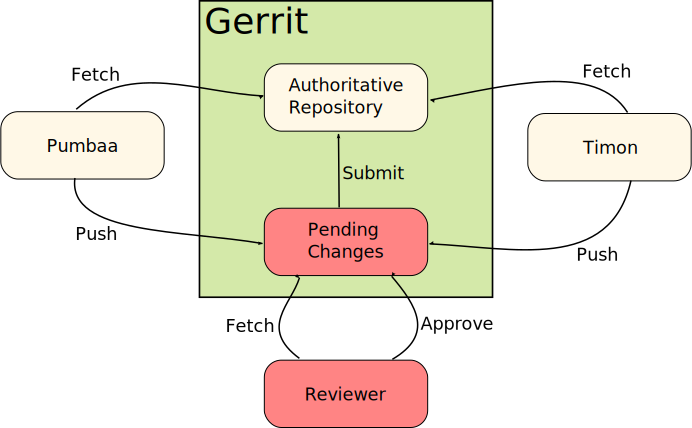
\includegraphics[height=7cm]{img/gerrit-workflow-gerrit.pdf}
\end{center}
\end{frame}

\begin{frame}{Gerrit and CI workflow}
  \begin{center}
    \includegraphics[height=7cm]{img/Git_gerrit_jenkins.png}
    \\ \tiny Courtesy of \url{http://blogs.collab.net/teamforge/teamforge-git-gerrit-integration-with-jenkins-ci}
  \end{center}
\end{frame}

\begin{frame}{Let's start}
  \begin{center}
    \includegraphics[height=2cm]{img/silvio-berlusconi.jpg}
  \end{center}
  \begin{itemize}
    \item \url{https://github.com/openstack}
    \item \url{https://github.com/stackforge}
    \item \url{http://devstack.org/}
  \end{itemize}
\end{frame}

\subsection{Sources}
\begin{frame}{Sources, code}
\begin{itemize}
  \item OpenStack Wiki\\\url{http://docs.openstack.org/trunk/}\\\url{http://nova.openstack.org/devref/}
  \item Images\\\url{http://ken.pepple.info/}\\\url{http://openstack.org/}
  \item Slides EmilienM and \url{https://github.com/sbadia/slides}
\end{itemize}
\end{frame}
